% BÀI TOÁN HÌNH HỌC - BAI_HINH_16 (TRÍCH ĐỀ 16)
\begin{ex}
% Câu 13
	Cho $\triangle ABC$ nhọn nội tiếp $(O)$. Hai đường cao $AN$ và $BM$ cắt nhau tại $H$.
	\begin{enumerate}
		\item[a)] Chứng minh: $M, H, N, C$ cùng thuộc một đường tròn.
		\item[b)] Vẽ $OP$ vuông góc với $BC$ ($P \in BC$). Gọi $G$ là giao điểm của $HO$ và $AP$.
		Chứng minh: $\widehat{HAB} = \widehat{OAC}$ và $G$ là trọng tâm của $\triangle ABC$.
	\end{enumerate}
\loigiai{
{
	\begin{center}
		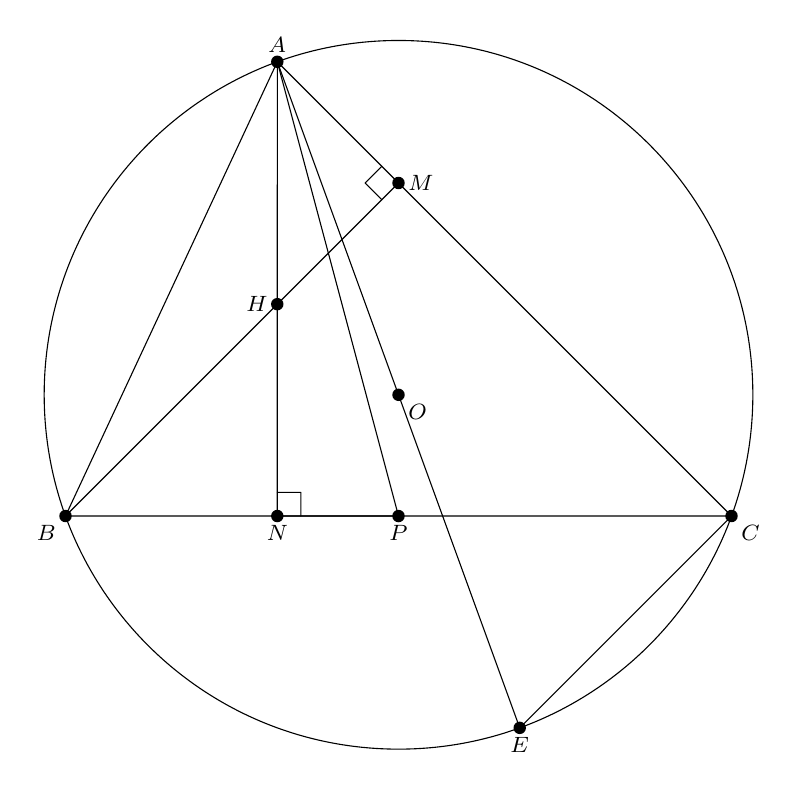
\begin{tikzpicture}[line join = round, line cap=round,>=stealth,font=\footnotesize,scale=1.5]
			\usetikzlibrary{calc,intersections,angles}
			
			% Khai báo hằng số
			\def\r{3} % r = 3cm
			
			% Định nghĩa tọa độ các điểm
			\coordinate (O) at (0,0);
			\coordinate (B) at (-160:\r); 
			\coordinate (C) at (-20:\r);  
			\coordinate (A) at (110:\r); 
			
			% N là hình chiếu của A lên BC
			\coordinate (N) at ($(B)!(A)!(C)$); % Bỏ _proj
			% M là hình chiếu của B lên AC
			\coordinate (M) at ($(A)!(B)!(C)$); % Bỏ _proj
			
			% H là giao điểm của AN và BM
			\path[name path=lineAN_H] (A) -- (N); % Sử dụng N
			\path[name path=lineBM_H] (B) -- (M); % Sử dụng M
			\path[name intersections={of=lineAN_H and lineBM_H, by=H}];
			
			% P là trung điểm của BC
			\coordinate (P) at ($(B)!0.5!(C)$);
			% Lấy điểm E sao cho O là trung điểm của AE (E = 2*O - A)
			\coordinate (E) at ($2*(O)-(A)$);
			
			% Vẽ các đối tượng hình học
			\draw (O) circle (\r);          % Đường tròn (O;r)
			\draw (A) -- (B) -- (C) -- cycle; % Tam giác A-B-C-A
			\draw (A) -- (E) -- (C);        % Đường A-E-C
			\draw (A) -- (P) -- (N) -- cycle; % Tam giác A-P-N (Sử dụng N)
			\draw (B) -- (M);            % Đoạn B-M (Sử dụng M)
			
			% Tô màu cho các điểm (theo cấu trúc đầu tiên)
			\fill (O) circle (1.5pt);
			\fill (A) circle (1.5pt);
			\fill (B) circle (1.5pt);
			\fill (C) circle (1.5pt);
			\fill (N) circle (1.5pt); % Sử dụng N
			\fill (M) circle (1.5pt); % Sử dụng M
			\fill (H) circle (1.5pt);
			\fill (P) circle (1.5pt);
			\fill (E) circle (1.5pt);
			
			% Đặt nhãn cho các điểm (theo cấu trúc đầu tiên)
			\node[below right] at (O) {$O$};
			\node[above] at (A) {$A$};
			\node[below left] at (B) {$B$};
			\node[below right] at (C) {$C$};
			\node[below] at (N) {$N$};      % Sử dụng N
			\node[right] at (M) {$M$};      % Sử dụng M
			\node[left] at (H) {$H$};      
			\node[below] at (P) {$P$};      
			\node[below] at (E) {$E$};      
			
			% Ký hiệu các góc vuông mới
			\pic[draw, angle radius=3mm]{right angle = A--N--C}; % Góc ANC (vuông tại N)
			\pic[draw, angle radius=3mm]{right angle = A--M--B}; % Góc AMB (vuông tại M)
			
		\end{tikzpicture}
		
	\end{center}
}
\end{ex}
